% Copyright 2004 by Till Tantau <tantau@users.sourceforge.net>.
%
% In principle, this file can be redistributed and/or modified under
% the terms of the GNU Public License, version 2.
%
% However, this file is supposed to be a template to be modified
% for your own needs. For this reason, if you use this file as a
% template and not specifically distribute it as part of a another
% package/program, I grant the extra permission to freely copy and
% modify this file as you see fit and even to delete this copyright
% notice. 

\documentclass{beamer}
\usepackage{amsmath,bm}
\usepackage{tikz}
\usetikzlibrary{arrows,automata}
\usepackage{graphicx}

\newcommand{\ssquare}{\text{\scalebox{0.6}{$\square$}}}
\newcommand{\U}{\bm{\mathcal{U}}}
% There are many different themes available for Beamer. A comprehensive
% list with examples is given here:
% http://deic.uab.es/~iblanes/beamer_gallery/index_by_theme.html
% You can uncomment the themes below if you would like to use a different
% one:
%\usetheme{AnnArbor}
%\usetheme{Antibes}
%\usetheme{Bergen}
%\usetheme{Berkeley}
%\usetheme{Berlin}
%\usetheme{Boadilla}
%\usetheme{boxes}
%\usetheme{CambridgeUS}
%\usetheme{Copenhagen}
%\usetheme{Darmstadt}
%\usetheme{default}
%\usetheme{Frankfurt}
%\usetheme{Goettingen}
%\usetheme{Hannover}
%\usetheme{Ilmenau}
%\usetheme{JuanLesPins}
%\usetheme{Luebeck}
\usetheme{Madrid}
%\usetheme{Malmoe}
%\usetheme{Marburg}
%\usetheme{Montpellier}
%\usetheme{PaloAlto}
%\usetheme{Pittsburgh}
%\usetheme{Rochester}
%\usetheme{Singapore}
%\usetheme{Szeged}
%\usetheme{Warsaw}

\title{A Discrete B\"uchi Automata Distance for Formal Methods Based Control}

% A subtitle is optional and this may be deleted
%\subtitle{Optional Subtitle}

%\author{F.~Author\inst{1} \and S.~Another\inst{2}}
\author{Garrett Thomas \\
Supervisor: Lars Lindemann \\
Examiner: Professor Dimos V. Dimarogonas}
% - Give the names in the same order as the appear in the paper.
% - Use the \inst{?} command only if the authors have different
%   affiliation.

\institute[Royal Institute of Technology, KTH] % (optional, but mostly needed)
{
  %\inst{1}%
  Automatic Control Department \\
  Royal Institute of Technology, KTH}
  %\and
  %\inst{2}%
  %Department of Theoretical Philosophy\\
  %University of Elsewhere}
% - Use the \inst command only if there are several affiliations.
% - Keep it simple, no one is interested in your street address.

\date{June $28^{\text{th}}$, 2017}
% - Either use conference name or its abbreviation.
% - Not really informative to the audience, more for people (including
%   yourself) who are reading the slides online

\subject{Buchi Distance}
% This is only inserted into the PDF information catalog. Can be left
% out. 

% If you have a file called "university-logo-filename.xxx", where xxx
% is a graphic format that can be processed by latex or pdflatex,
% resp., then you can add a logo as follows:

% \pgfdeclareimage[height=0.5cm]{university-logo}{university-logo-filename}
% \logo{\pgfuseimage{university-logo}}

% Delete this, if you do not want the table of contents to pop up at
% the beginning of each subsection:
\AtBeginSubsection[]
{
  \begin{frame}<beamer>{Outline}
    \tableofcontents[currentsection,currentsubsection]
  \end{frame}
}

% Let's get started
\begin{document}

\begin{frame}
  \titlepage
\end{frame}

\begin{frame}{Outline}
  \tableofcontents
  % You might wish to add the option [pausesections]
\end{frame}

% Section and subsections will appear in the presentation overview
% and table of contents.
\section{Problem and Motivation}

\subsection{Formal Methods Based Control}

\begin{frame}{Linear Temporal Logic}
  \begin{itemize}
  \item {
    We will be using \textbf{Linear Temporal Logic (LTL)}, defined recursively as
    $\varphi ::= \top | \alpha | \neg \varphi_1 | \varphi_1  \lor \varphi_2 | \textbf{X} \varphi_1 | \varphi_1 \bm{\mathcal{U}} \varphi_2$
    \pause
  }
  \item {
    Why?LTL formulas are versatile; LTL allows us to encode statements about the robot and workspace, and also how events relate to each other in the time domain. \\
    Ex. from \cite{guo15} $ \varphi= \diamond(\text{rball} \land \diamond \text{basket}) \land \diamond \ssquare \text{r1}$ \\
    "Eventually pick up the red ball and put it in one of the baskets. Then go home to r1" \\
     \centering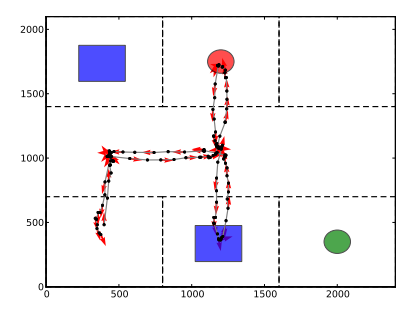
\includegraphics[scale=0.3]{ltlExampleWorkspace}\par
  }
  \end{itemize}
\end{frame}

\begin{frame}{LTL Motion and Task Planning}
	\begin{itemize}	
	\item {
		LTL Motion and task planning is done in three Steps \cite{belta07}
		\pause
	}
	\item<2->{
		Specification: Create a graph (the \textit{product automaton}) based on the workspace, robot motion, and LTL formula such that all paths in this graph satisfy the specification.
	}
	\item<3->{
		Execution: Find a discrete path in this graph using an optimality criterion.*
	}
	\item<4->{
		Implementation: Calculate the continuous controllers such that the continuous path will satisfy the discrete path.
	}
	\end{itemize}	
	
\end{frame}
\subsection{The Product Automaton}

% You can reveal the parts of a slide one at a time
% with the \pause command:
\begin{frame}{Finite-State Transition System}
  \begin{itemize}
  \item<1->{
    The product automaton is the of a \textit{finite-state transition system} and a \textit{B\"uchi automaton}
    \pause % The slide will pause after showing the first item
  }
  \end{itemize}
    \begin{block}{Finite-State Transition System (FTS)}
	\small An FTS is a tuple $\mathcal{T} = (\Pi, \rightarrow, \Pi_0, AP,L_D)$ where $\Pi$ is the set of states, $\rightarrow \subseteq \Pi \times \Pi$ is the transitions, $\Pi_0 \subseteq \Pi$ is the initial state(s), $AP$ is the set of atomic propositions, and $L: \Pi \rightarrow 2^{AP}$ is the labelling function (goes from a state to the set of atomic propositions that are true in that state).
	\end{block}
  
    
%  \item<5-> {
%    Fifth item. \uncover<6->{Extra text in the fifth item.}
%  }
  \begin{figure}
\centering
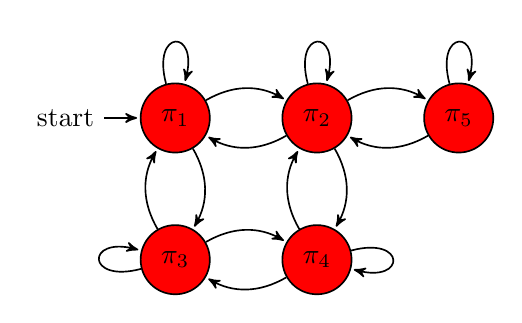
\begin{tikzpicture}[->,>=stealth',shorten >=1pt,auto,node distance=1.8cm,
                    semithick]
  \tikzstyle{every state}=[fill=red,draw=black,text=black]

  \node[initial,state] (A)                    { $\pi_1$};
  \node[state]         (B) [ right of=A] { $\pi_2$};
  \node[state]         (C) [below of=A] { $\pi_3$};
  \node[state]         (D) [right of=C] { $\pi_4$};
  \node[state]         (E) [right of=B] { $\pi_5$};

  \path (A) edge     [bend left]        (B)
  		(B) edge     [bend left]           (A)
		(A) edge     [bend left]         (C)
  		(C) edge     [bend left]           (A)
  		(C) edge     [bend left]         (D)
  		(D) edge     [bend left]           (C)
  		(B) edge     [bend left]           (D)
  		(D) edge     [bend left]           (B)
  		(B) edge     [bend left]           (E)
  		(E) edge     [bend left]           (B)
        (A) edge [loop above]   (A)
        (B) edge [loop above]   (B)
        (C) edge [loop left]  (C)
        (D) edge [loop right]  (D)
        (E) edge [loop above]  (E);
\end{tikzpicture}

\label{fig:ftsEx}
\end{figure}
\end{frame}

\begin{frame}{B\"uchi Automaton}
\begin{block}{B\"uchi Automaton}
	\small A B\"uchi automaton is a tuple $\mathcal{A}_\varphi = (\mathcal{Q},2^{AP},\delta,\mathcal{Q}_0,\mathcal{F})$ where $\mathcal{Q}$ is a finite set of states, $\mathcal{Q}_0 \subseteq \mathcal{Q}$ is the set of initial states, $2^{AP}$ is the alphabet, $\delta: \mathcal{Q} \times 2^{AP} \rightarrow 2^\mathcal{Q}$ is a transition relation, and $\mathcal{F} \subseteq \mathcal{Q}$ is the set of accepting states.
	\end{block}

	\begin{itemize}
	\item {
	A path on a B\"uchi automaton is accepting if it passes through an accepting state infinitely many times.
	}
	\item {
	For any LTL formula $\varphi$ over $AP$, there exists a B\"uchi automaton over $2^{AP}$ corresponding to $\varphi$ \cite{baier08}
	}
	\end{itemize}
	Reachability while avoiding regions $\varphi = \neg(\pi_3 \lor \pi_4) \U \pi_5$
	
	\begin{figure}
\centering
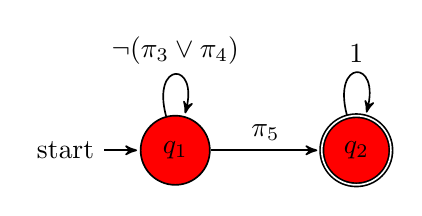
\begin{tikzpicture}[->,>=stealth',shorten >=1pt,auto,node distance=2.3cm,
                    semithick]
  \tikzstyle{every state}=[fill=red,draw=black,text=black]

  \node[initial,state] (A)                    {$q_1$};
  \node[state,accepting]         (B) [right of=A] {$q_2$};

  \path (A) edge              node {$\pi_{5}$} (B)
  		(A) edge [loop above] node {$\neg( \pi_3 \lor \pi_4) $} (A)
  		(B) edge [loop above] node {$1$} (B);
\end{tikzpicture}
\end{figure}
\end{frame}


\subsection{Another Subsection}

\begin{frame}{Blocks}
\begin{block}{Block Title}
You can also highlight sections of your presentation in a block, with it's own title
\end{block}
\begin{theorem}
There are separate environments for theorems, examples, definitions and proofs.
\end{theorem}
\begin{example}
Here is an example of an example block.
\end{example}
\end{frame}

% Placing a * after \section means it will not show in the
% outline or table of contents.
\section*{Summary}

\begin{frame}{Summary}
  \begin{itemize}
  \item
    The \alert{first main message} of your talk in one or two lines.
  \item
    The \alert{second main message} of your talk in one or two lines.
  \item
    Perhaps a \alert{third message}, but not more than that.
  \end{itemize}
  
  \begin{itemize}
  \item
    Outlook
    \begin{itemize}
    \item
      Something you haven't solved.
    \item
      Something else you haven't solved.
    \end{itemize}
  \end{itemize}
\end{frame}



% All of the following is optional and typically not needed. 
\appendix
\section<presentation>*{\appendixname}
\subsection<presentation>*{For Further Reading}

\begin{frame}[allowframebreaks]
  \frametitle<presentation>{For Further Reading}
    
  \begin{thebibliography}{10}
    
  \beamertemplatebookbibitems
  % Start with overview books.

  \bibitem{Author1990}
    A.~Author.
    \newblock {\em Handbook of Everything}.
    \newblock Some Press, 1990.
 
    
  \beamertemplatearticlebibitems
  % Followed by interesting articles. Keep the list short. 

  \bibitem{Someone2000}
    S.~Someone.
    \newblock On this and that.
    \newblock {\em Journal of This and That}, 2(1):50--100,
    2000.
  \end{thebibliography}
\end{frame}

\begin{frame}[allowframebreaks]
        \frametitle{References}
        \bibliographystyle{amsalpha}
        \bibliography{../writing/bibliography}
\end{frame}

\end{document}